\documentclass{article}
\usepackage{graphicx} % Required for inserting images
\usepackage{wrapfig}
\usepackage{subcaption}
\usepackage{listings}
\usepackage{float}
\usepackage{xcolor}
\graphicspath{{./images/}}

\definecolor{codegreen}{rgb}{0,0.6,0}
\definecolor{codegray}{rgb}{0.5,0.5,0.5}
\definecolor{codepurple}{rgb}{0.58,0,0.82}
\definecolor{backcolour}{rgb}{0.95,0.95,0.92}

\lstdefinestyle{mystyle}{
    backgroundcolor=\color{backcolour},   
    commentstyle=\color{codegreen},
    keywordstyle=\color{magenta},
    numberstyle=\tiny\color{codegray},
    stringstyle=\color{codepurple},
    basicstyle=\ttfamily\footnotesize,
    breakatwhitespace=false,         
    breaklines=true,                 
    captionpos=b,                    
    keepspaces=true,                 
    numbers=left,                    
    numbersep=5pt,                  
    showspaces=false,                
    showstringspaces=false,
    showtabs=false,                  
    tabsize=2
}

\lstset{style=mystyle}


\usepackage[backend=biber, style=apa, sorting=nyt]{biblatex}
\addbibresource[]{./ref.bib}

\title{Advanced Maths Documentation}
\author{Thomas Lower}
\date{January 2024}

\begin{document}

\maketitle

\pagebreak

\section{Task A} \label{a}

\begin{figure}[h]
    \centering
    \caption{The starting image}
    \label{fig:start}
    \includegraphics[width=0.5\textwidth]{start_image.png}
\end{figure}

\begin{figure}[h]
    \centering
    \caption{The starting image set to greyscale}
    \label{fig:greyscale}
    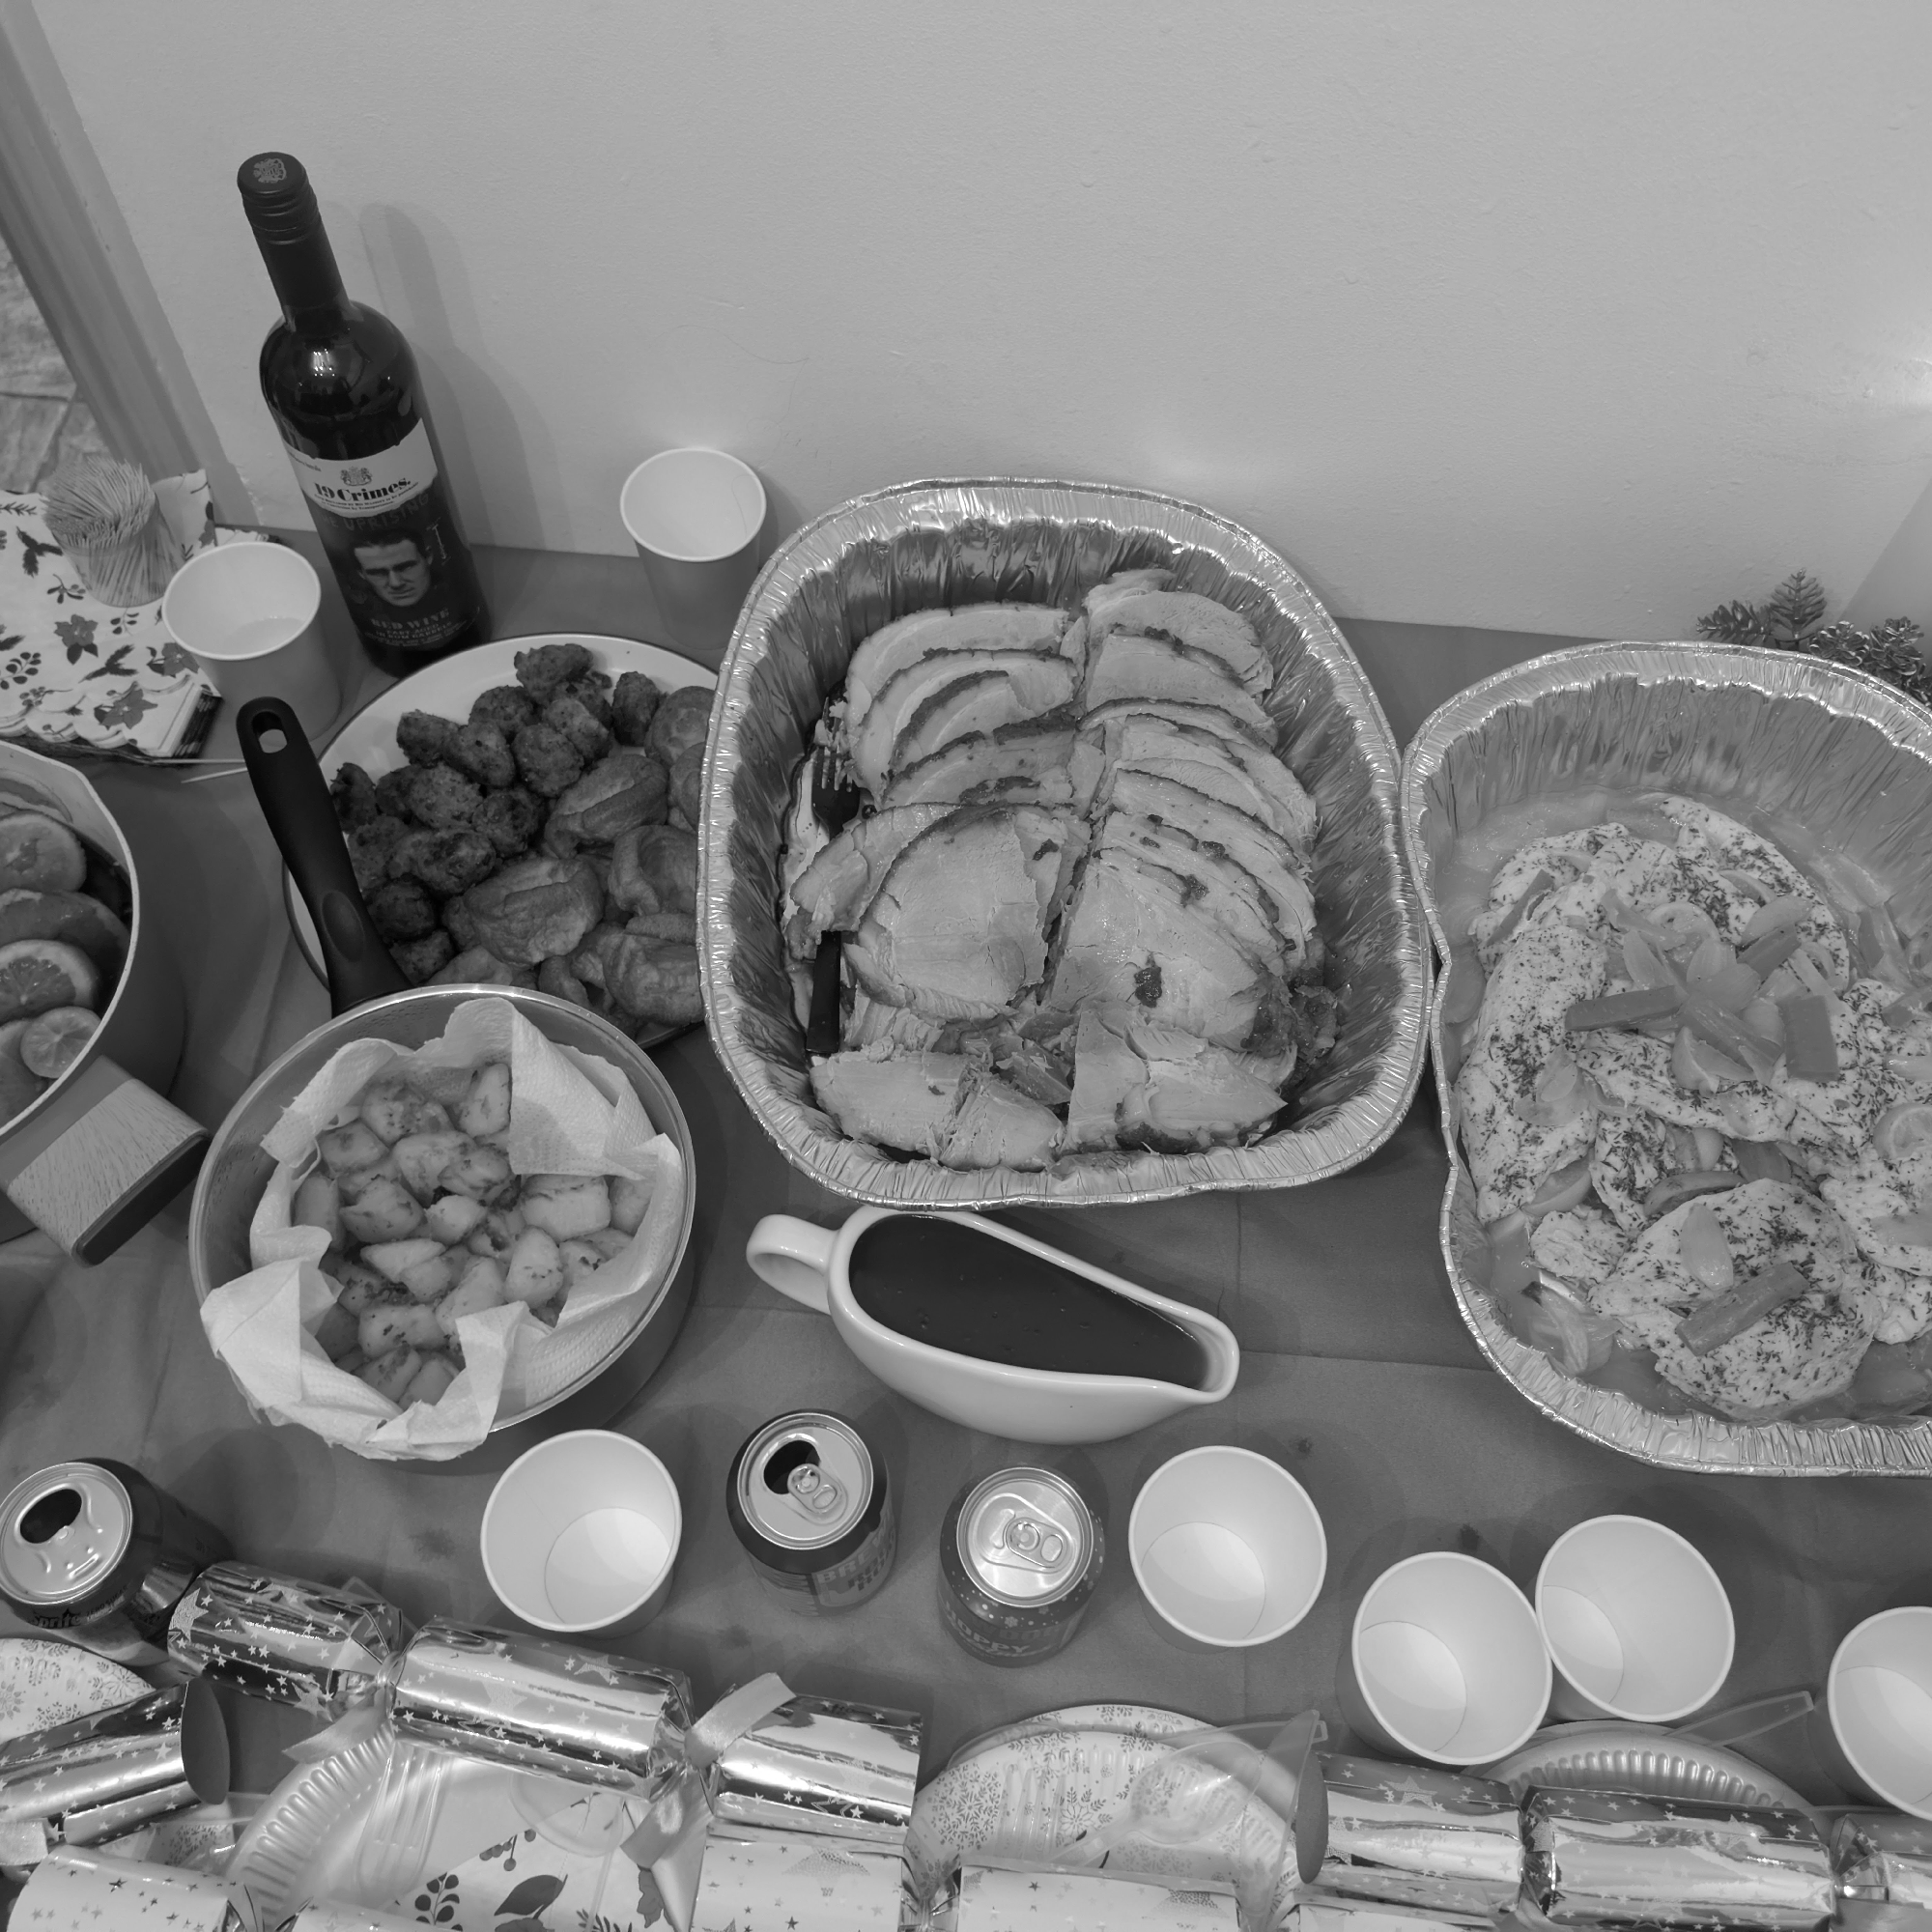
\includegraphics[width=0.5\textwidth]{grayscale_image.png}
\end{figure}

The image in figure \ref{fig:start} is a coloured image of our course's Christmas dinner. It is pre-cropped to fit the aspect ratio of the program is scaled within the program to fit the window.

In preparation for the task in section \ref{b}, the program will convert the image to greyscale before saving it back to disk. The algorithm used for this is a basic mean average of the 3 colour channels. The result of which is figure \ref{fig:greyscale}.

.BMP files are used throughout this project due to their lack of compression and clarity of pixel data that would allow maximum control over the given pixel data.

All images are scaled to be 2000 x 2000.

\section{Task B} \label{b}

\begin{figure}[h]
    \centering
    \caption{The result of the first Fourier transform}
    \label{fig:fourier}
    
\includegraphics[width=0.5\textwidth]{fourier_image.png}
\end{figure}

When Fourier transforming figure \ref{fig:greyscale}, the resultant image can be seen in \ref{fig:fourier}. When Inversely Fourier transformed, this recreated figure \ref{fig:greyscale} almost exactly.

The system treats this process as a series of unrelated steps as to avoid data from a previous step contaminating that of the next step (such as a Fourier transform being affected by data from a previous Fourier transform). It reads each pixel from the greyscale screen and divides it by 255 to give a normalized value. This is then stored in a 2 dimensional array (an array of rows, each row being an array of floating point complex numbers) with the normalized values from the greyscale being used as the real value of a complex number which is passed into the Fourier transform function.

The Fourier function itself then reads in the entire row, calculates the angle for the given pixel in the row, applies the exponent of the pixel as the imaginary part of the complex number and scales the entire pixel by the size of the row (see section \ref{a} for sizes). An output array is then created in the heap (rather than the call stack) so that a pointer to the array can be returned.

Afterwards, the Inverse Fourier transform function is applied in a similar fashion but with 2 differences: The angle is inverted, and the result is not scaled. I opted to write this as a separate function to avoid confusion and make it clearer to myself which way I was Fourier transforming.

Both transforms make sure to return the entire complex number and then only use the absolute value of this for rendering to the screen and image while saving the rest for future calculations to avoid truncation of data.

\section{Task C} \label{c}

\begin{figure}[h]
    \centering
    \caption{The result of the 2D Fourier transform}
    \label{fig:2d}
    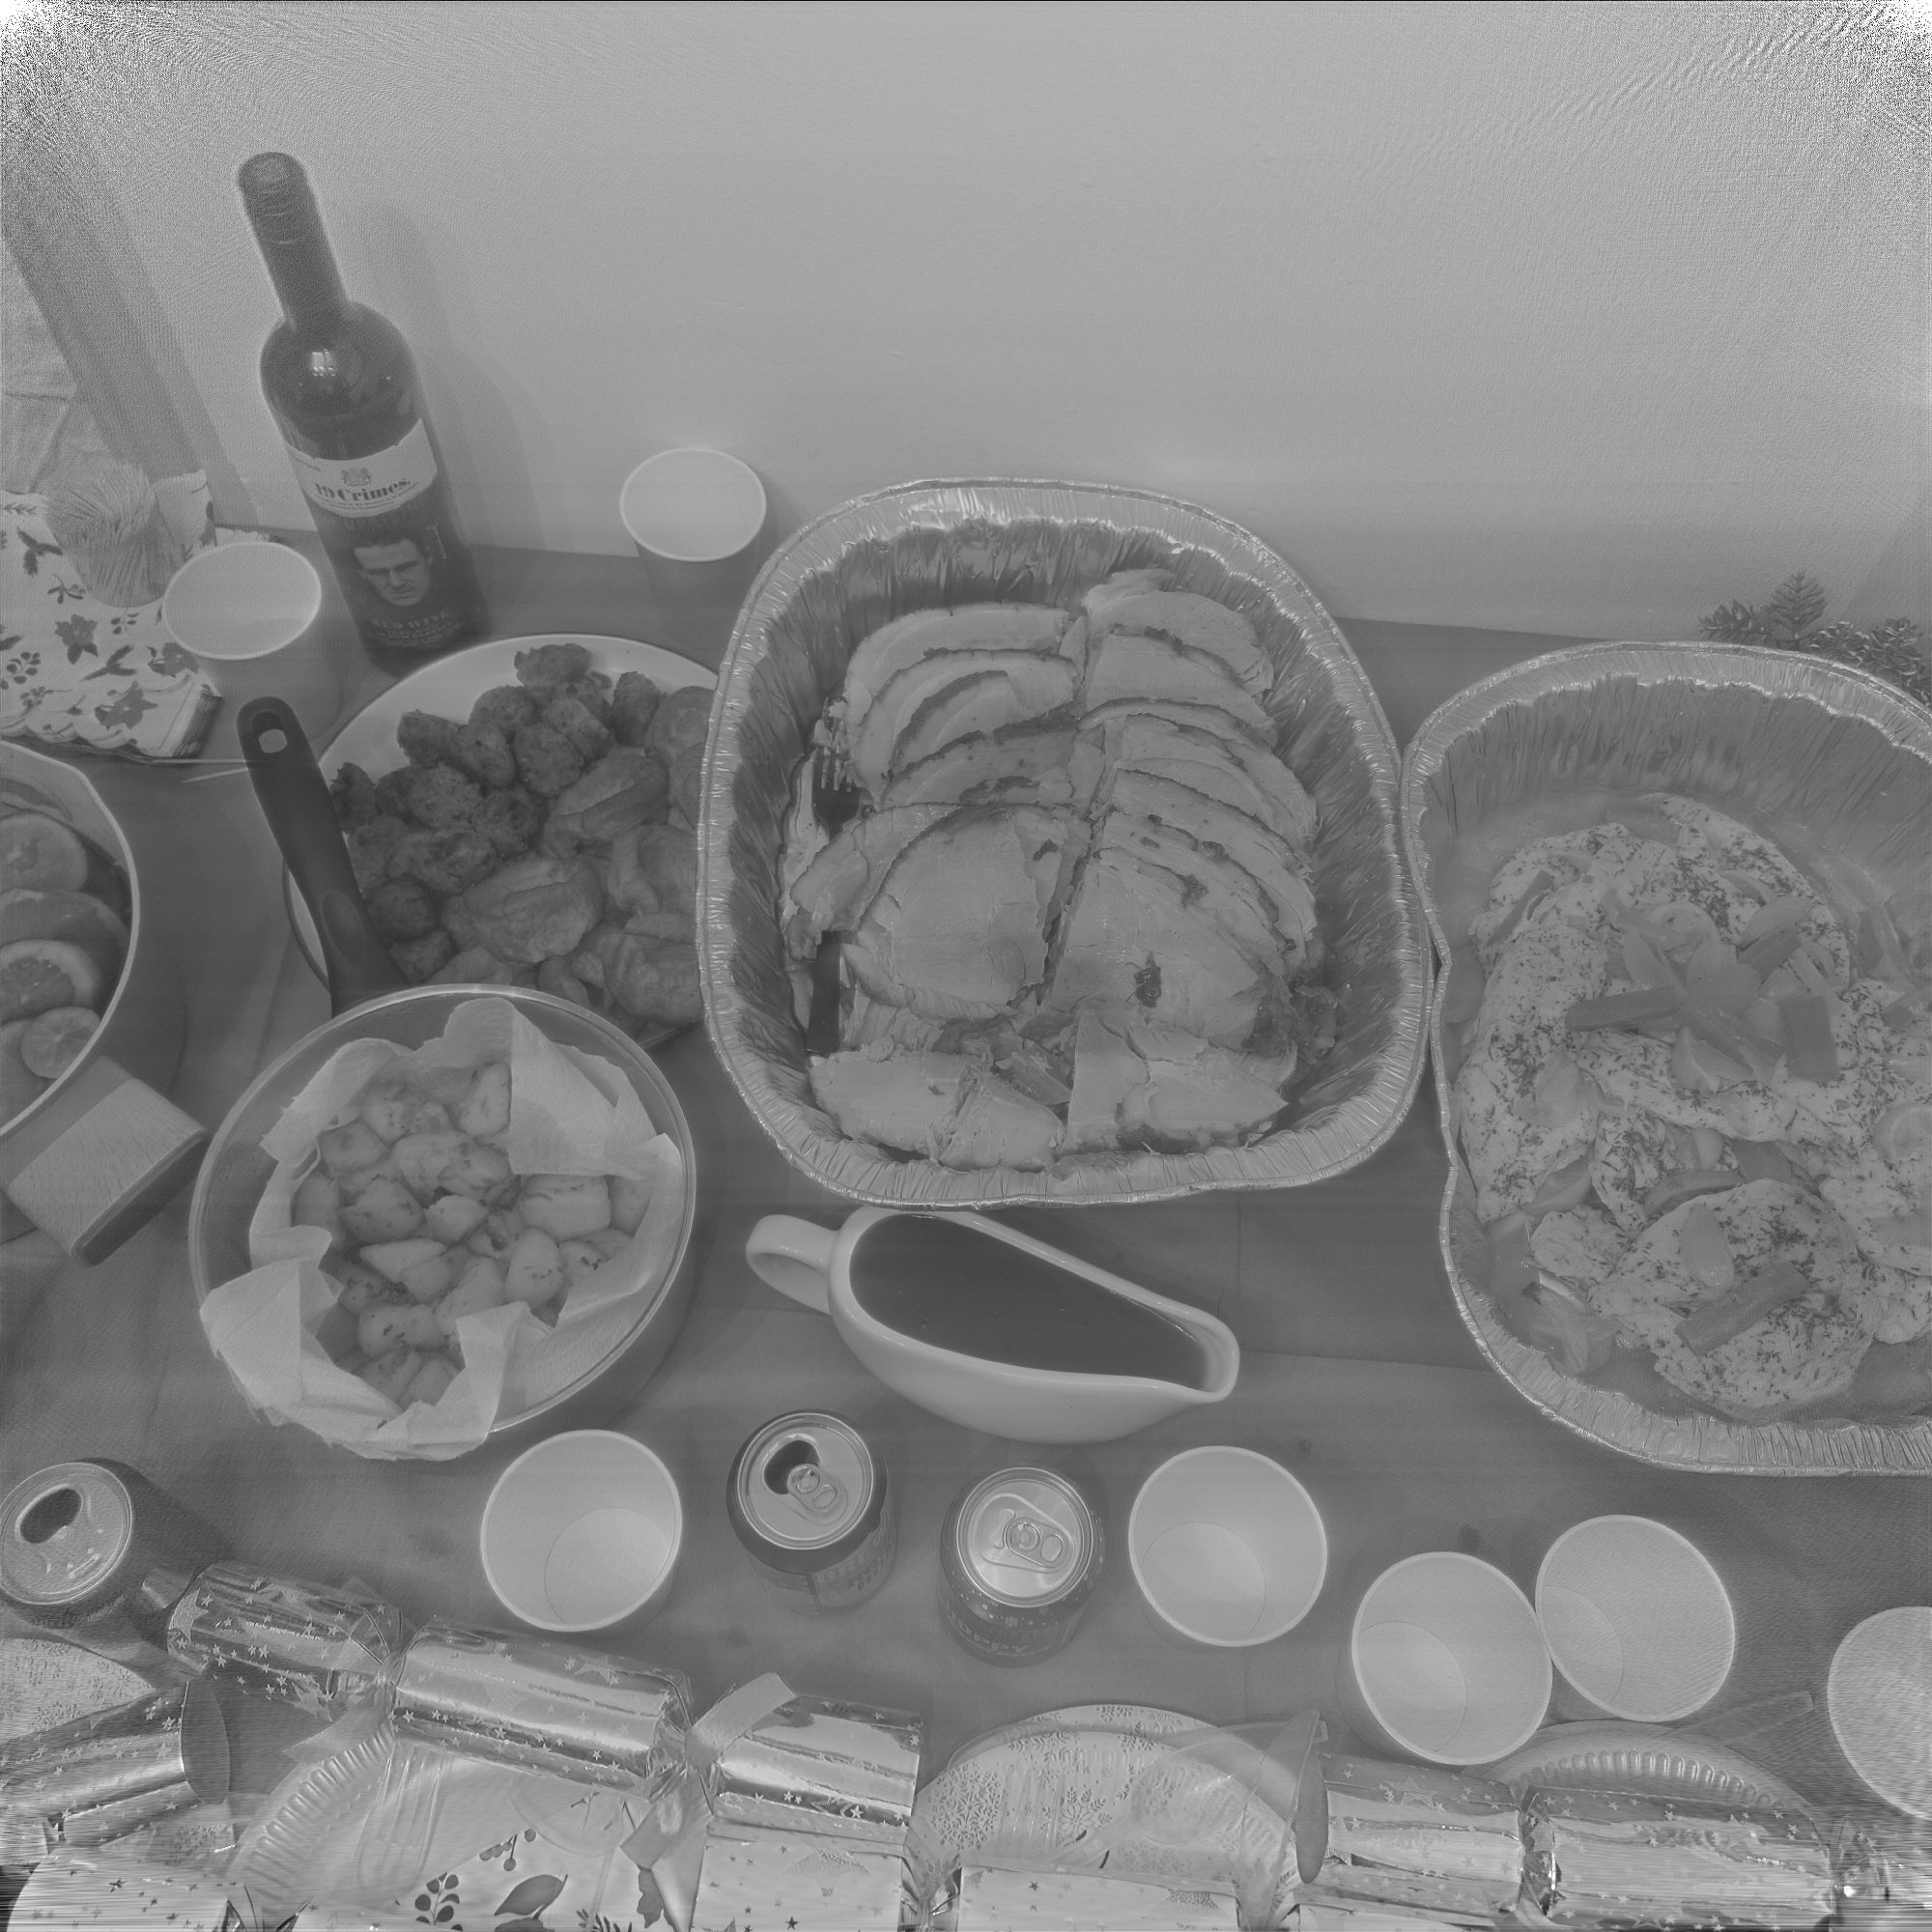
\includegraphics[width=0.5\textwidth]{double_fourier_image.png}
\end{figure}

To swap the rows and columns of the Fourier transform result, the algorithm simply looks through the entire 2D array polynomially and swaps \verb|result[x][y] with result[y][x]|. The result of this is then inversely Fourier transformed to simulate a 2D Fourier transform. The resultant image figure \ref{fig:2d} features the same image but with a grey undertone as well as white artefacts in the top corners and black artefacts in the bottom corners.

\section{Task D} \label{d}

\begin{figure}[H]
    \centering
    \caption{The box convolution kernal}
    \label{fig:box}
    
\includegraphics[width=0.5\textwidth]{rect_image.png}
\end{figure}

\begin{figure}[H]
    \centering
    \caption{The result of Fourier transforming the box convolution kernal}
    \label{fig:fourierBox}
    
\includegraphics[width=0.5\textwidth]{fourier_rect_image.png}
\end{figure}

\begin{figure}[H]
    \centering
    \caption{The result of multiplying the kernal with the fourier transformed image}
    \label{fig:boxMultiply}
    
\includegraphics[width=0.5\textwidth]{convolution_image.png}
\end{figure}

\begin{figure}[H]
    \centering
    \caption{The result of inversely transforming figure \ref{fig:boxMultiply}}
    \label{fig:fourierMultiply}
    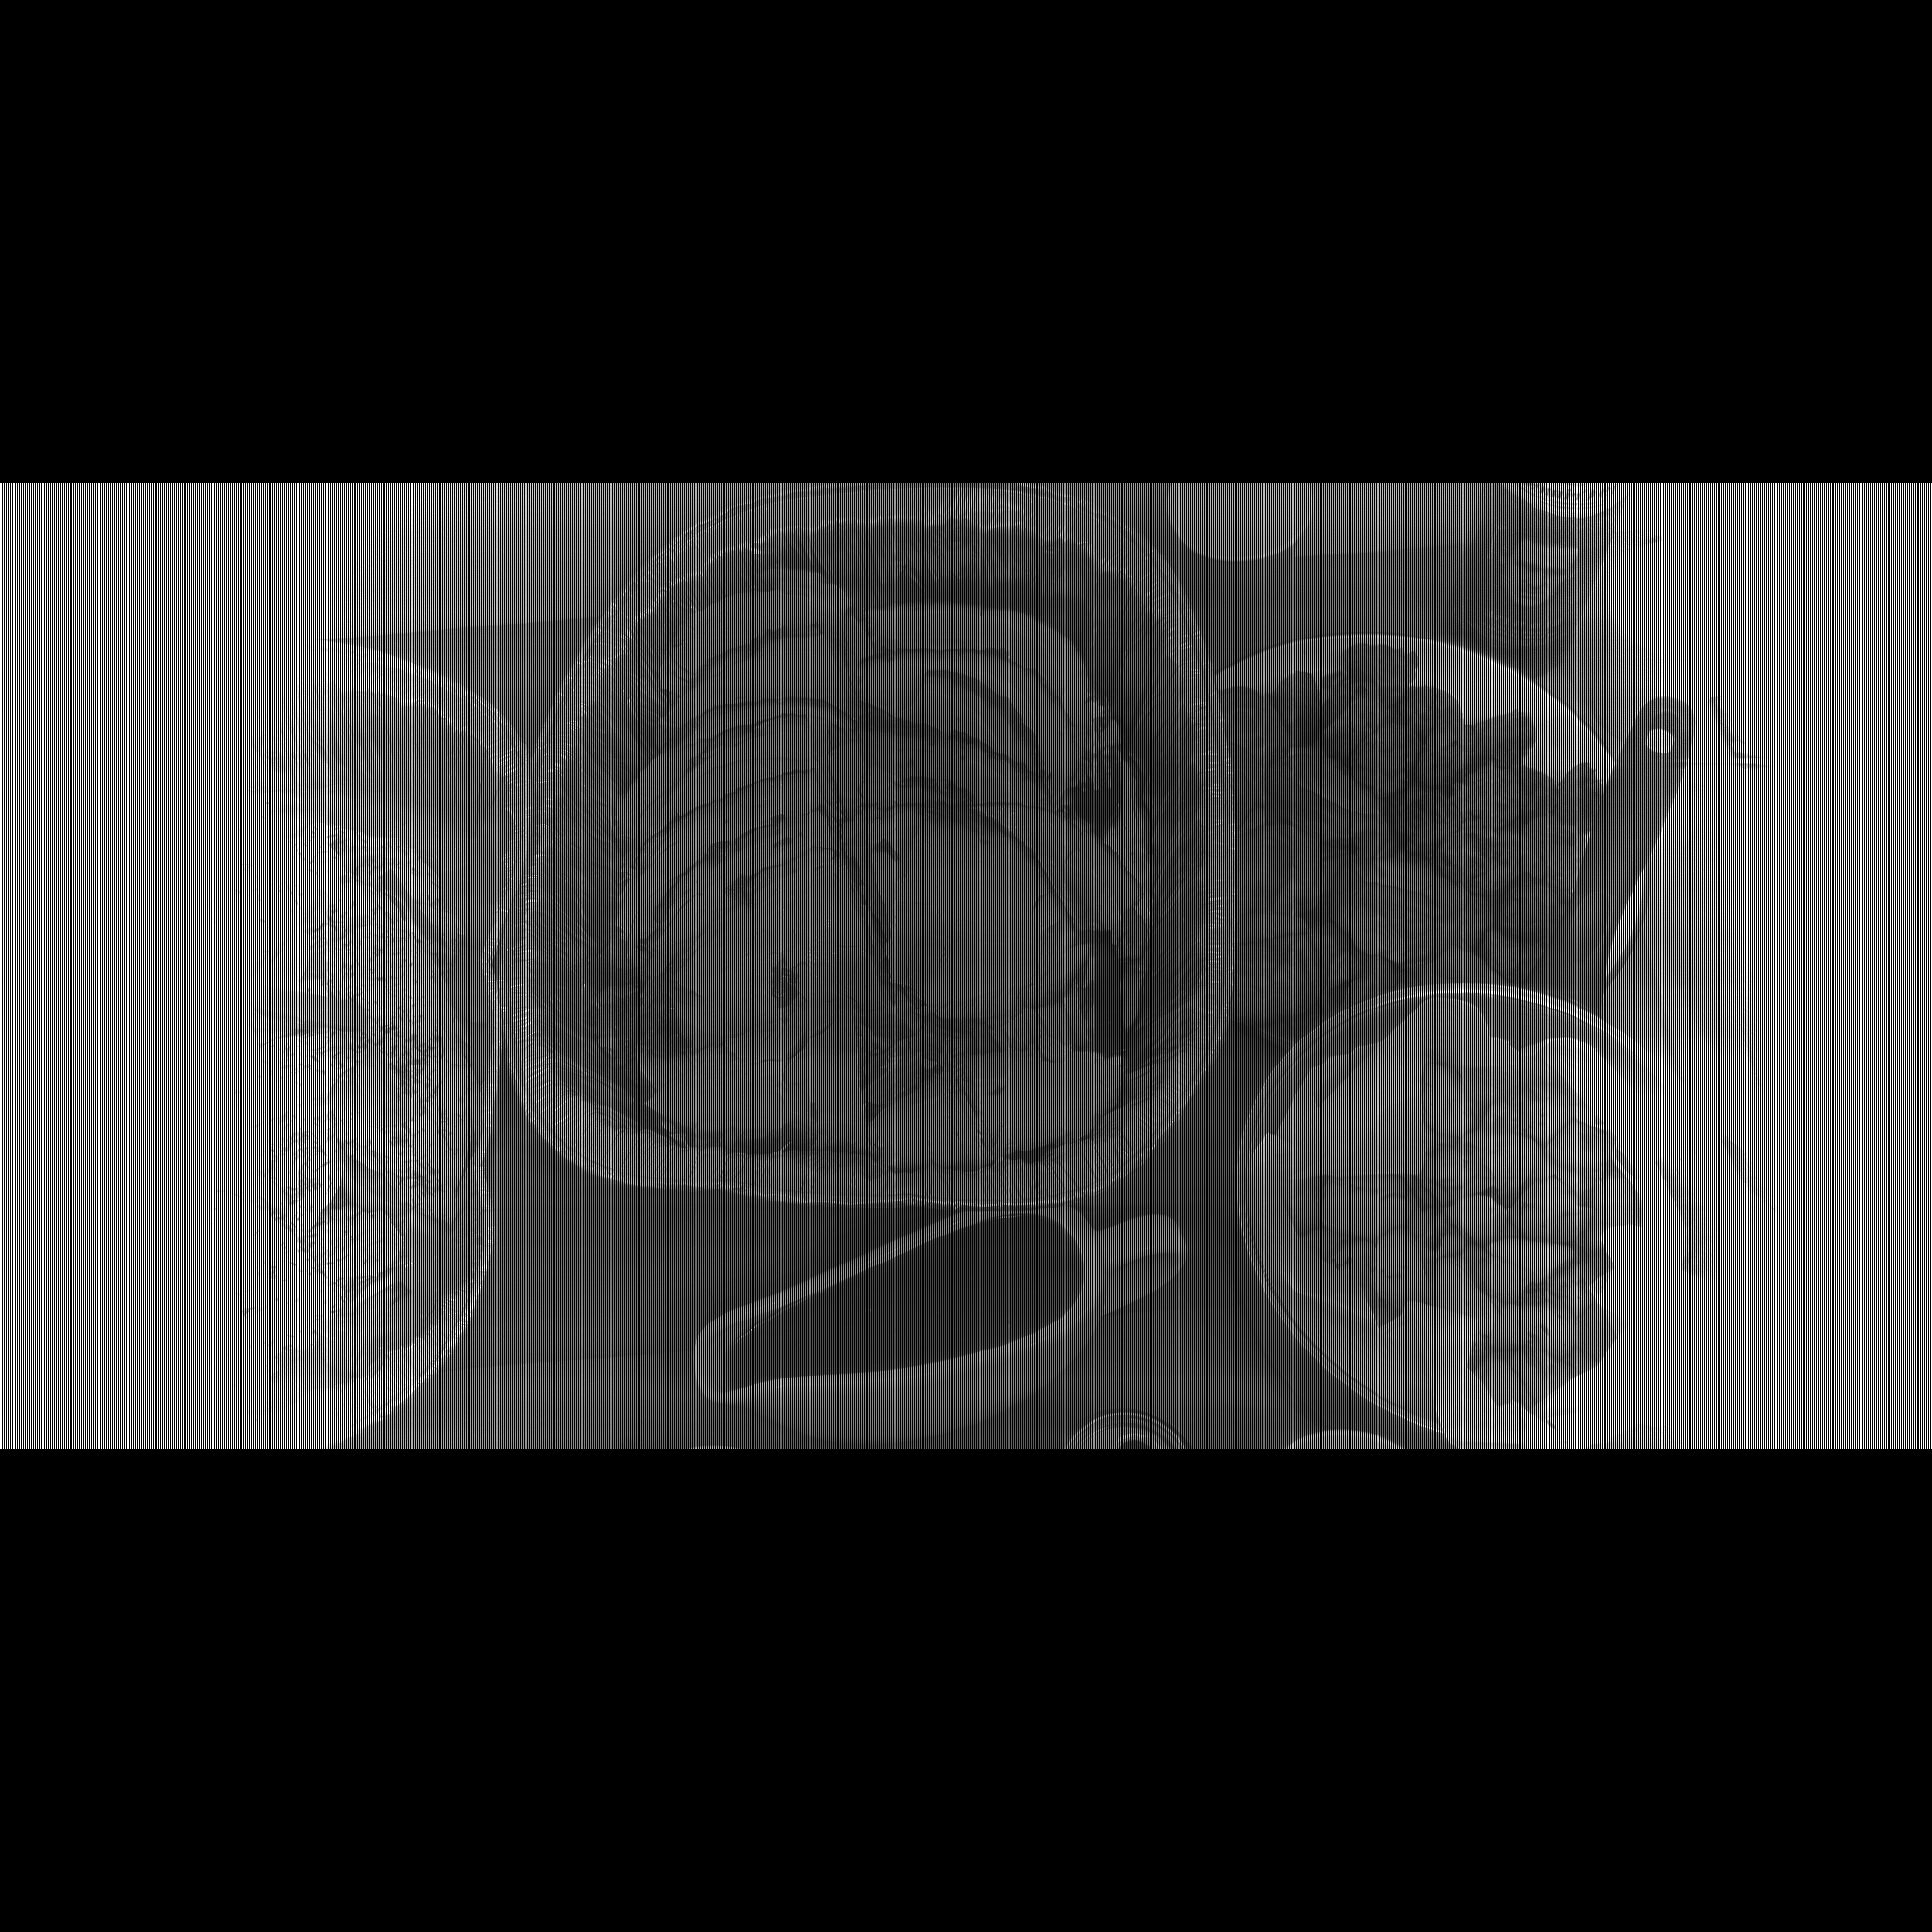
\includegraphics[width=0.5\textwidth]{double_inverse_fourier_image.png}
\end{figure}

This algorithm applies a convolution box to the image. The box is sized to take up \verb|50%| of the screen and be centred in the middle, as visible in figure \ref{fig:box}. The box is then fourier transformed to produce figure \ref{fig:fourierBox} and multiplied with the intermediate of the 2D Fourier transform in section \ref{c}. The result of this multiplication is \ref{fig:boxMultiply} which when inversely Fourier transformed created \ref{fig:fourierMultiply}.

Multiplication is used rather than direct convolution due to the idea that "Convolution in time domain is multiplication in the frequency domain" \parencite{ian1}.

\section{Task E} \label{e}


\begin{figure}[H]
    \centering
    \caption{The box convolution kernal}
    \label{fig:box2}
    
\includegraphics[width=0.5\textwidth]{rect_image2.png}
\end{figure}

\begin{figure}[H]
    \centering
    \caption{The result of Fourier transforming the box convolution kernal}
    \label{fig:fourierBox2}
    
\includegraphics[width=0.5\textwidth]{fourier_rect_image2.png}
\end{figure}

\begin{figure}[H]
    \centering
    \caption{The result of multiplying the kernal with the fourier transformed image}
    \label{fig:boxMultiply2}
    
\includegraphics[width=0.5\textwidth]{convolution_image2.png}
\end{figure}

\begin{figure}[H]
    \centering
    \caption{The result of inversely transforming figure \ref{fig:boxMultiply2}}
    \label{fig:fourierMultiply2}
    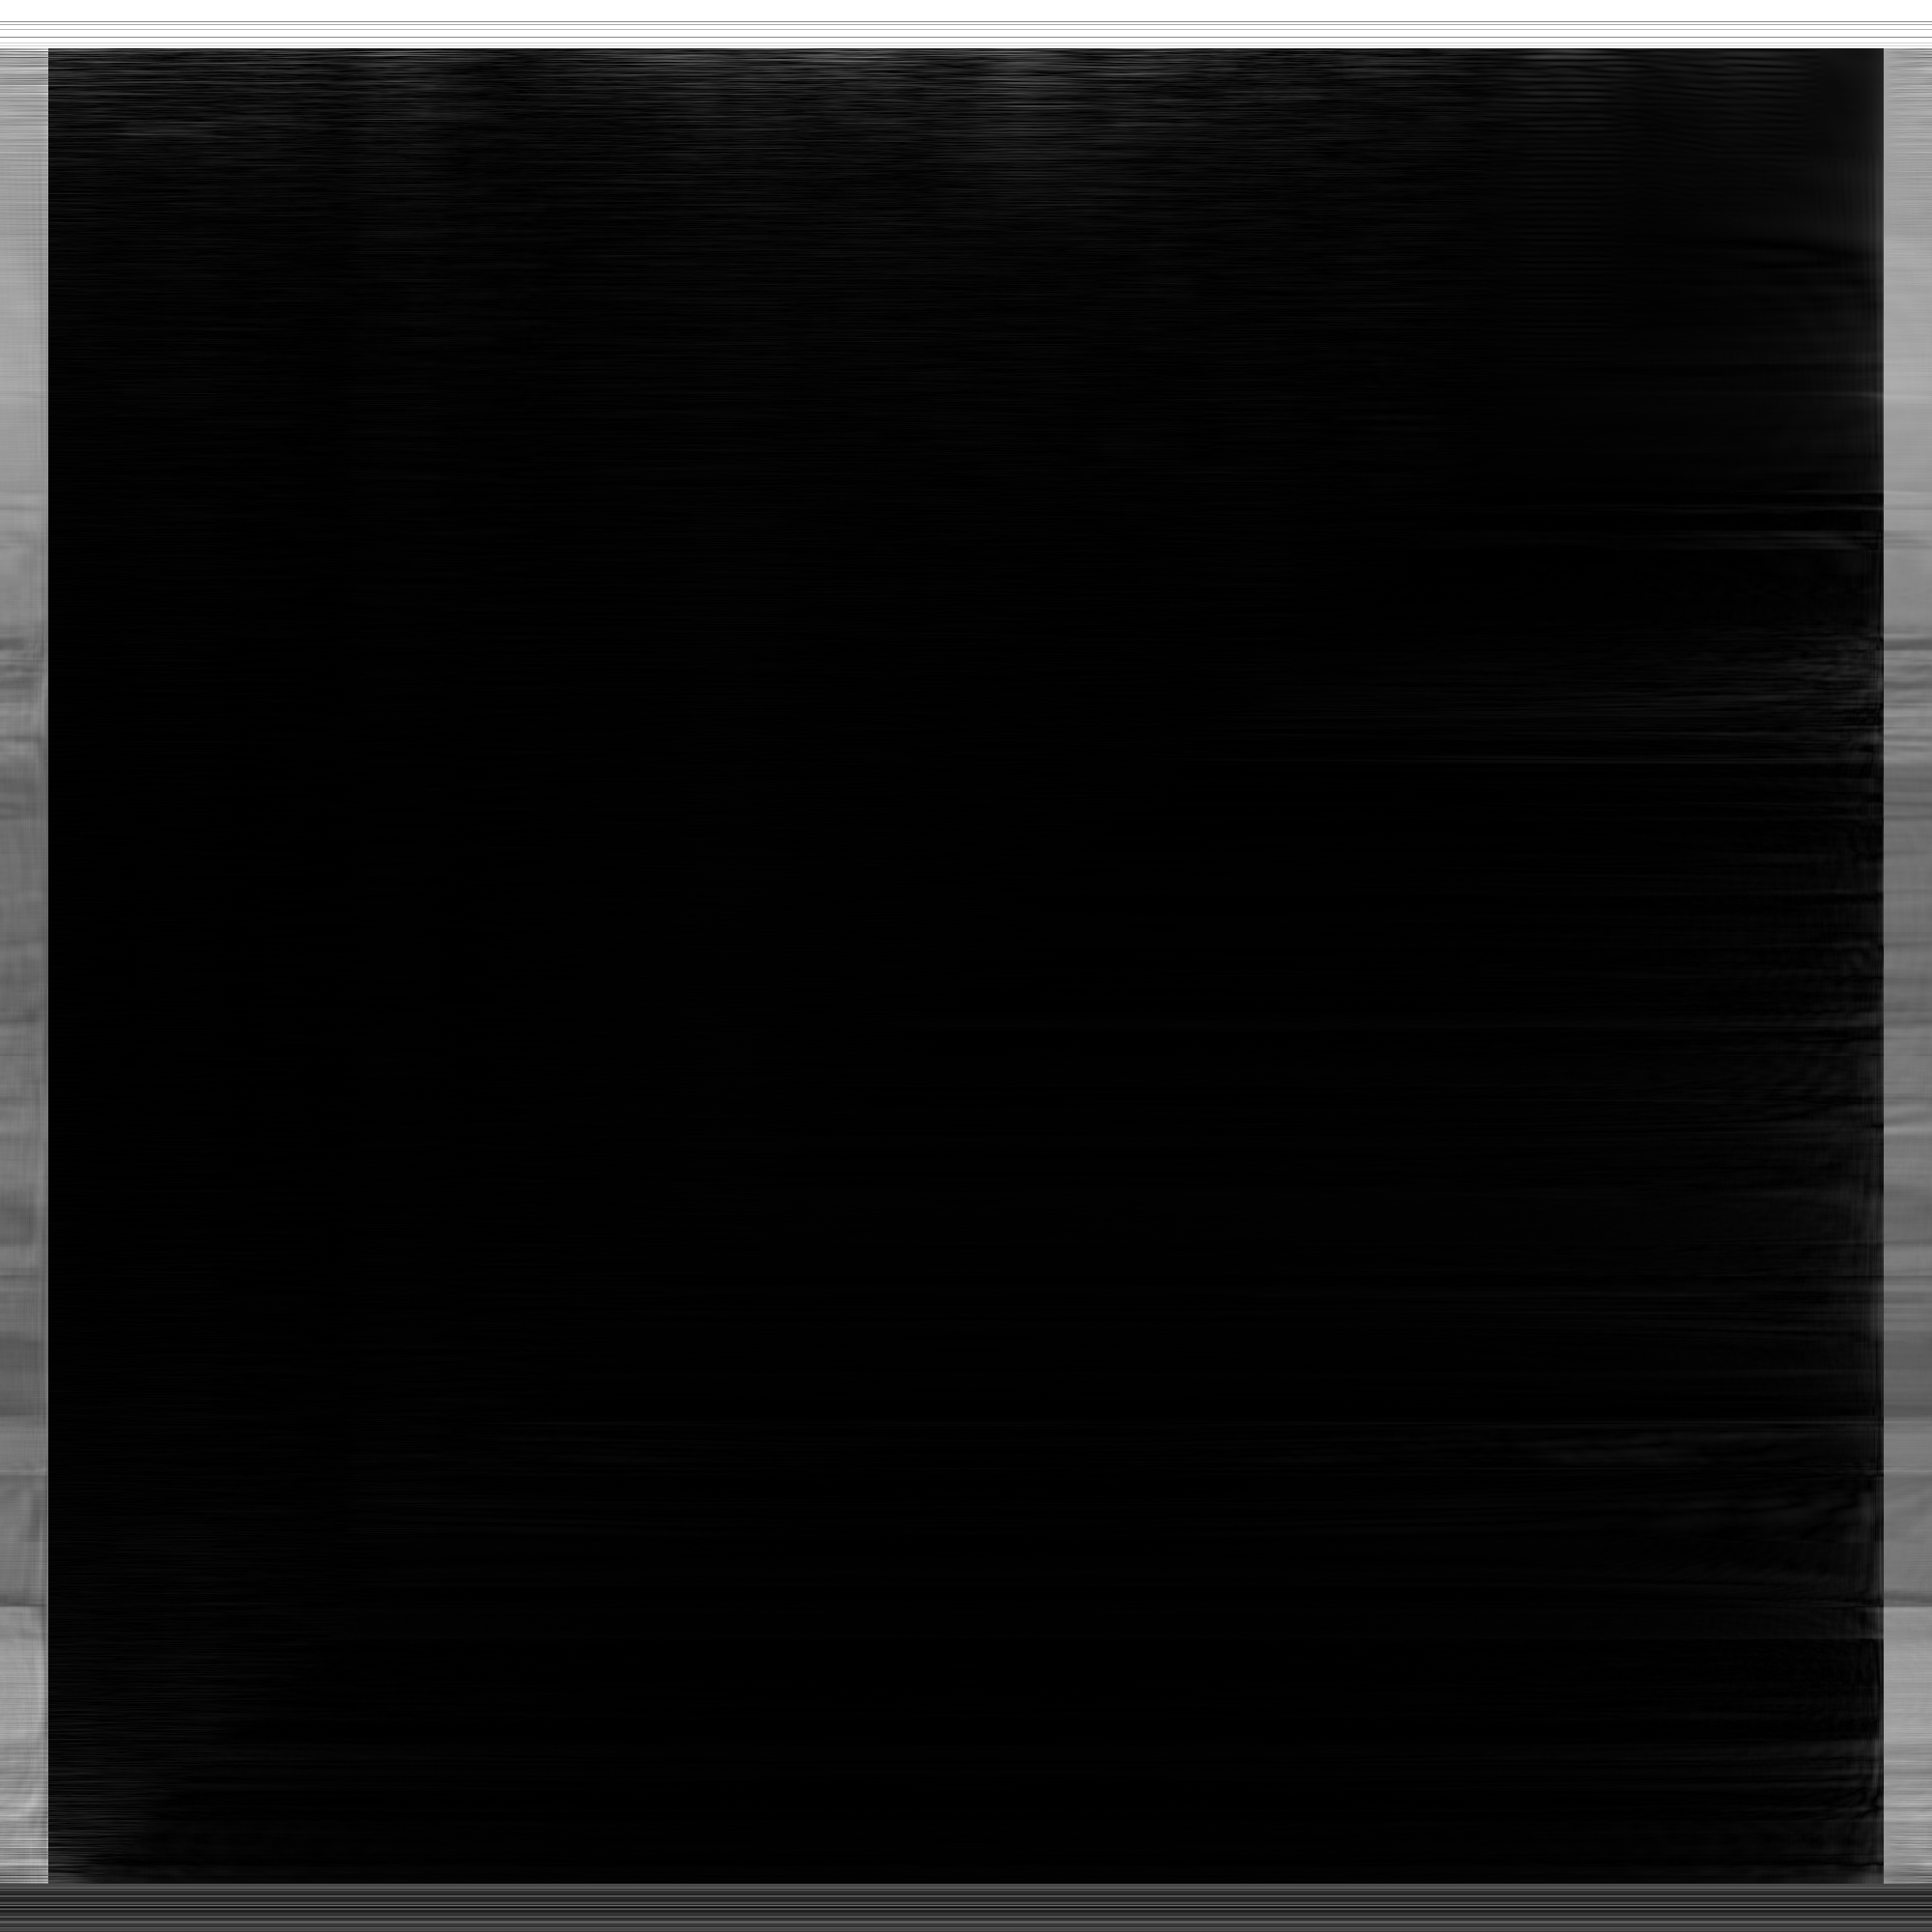
\includegraphics[width=0.5\textwidth]{inverse_fourier_image2.png}
\end{figure}

\begin{figure}[H]
    \centering
    \caption{The result of inversely transforming figure \ref{fig:fourierMultiply2}}
    \label{fig:fourierTransformFinal}
    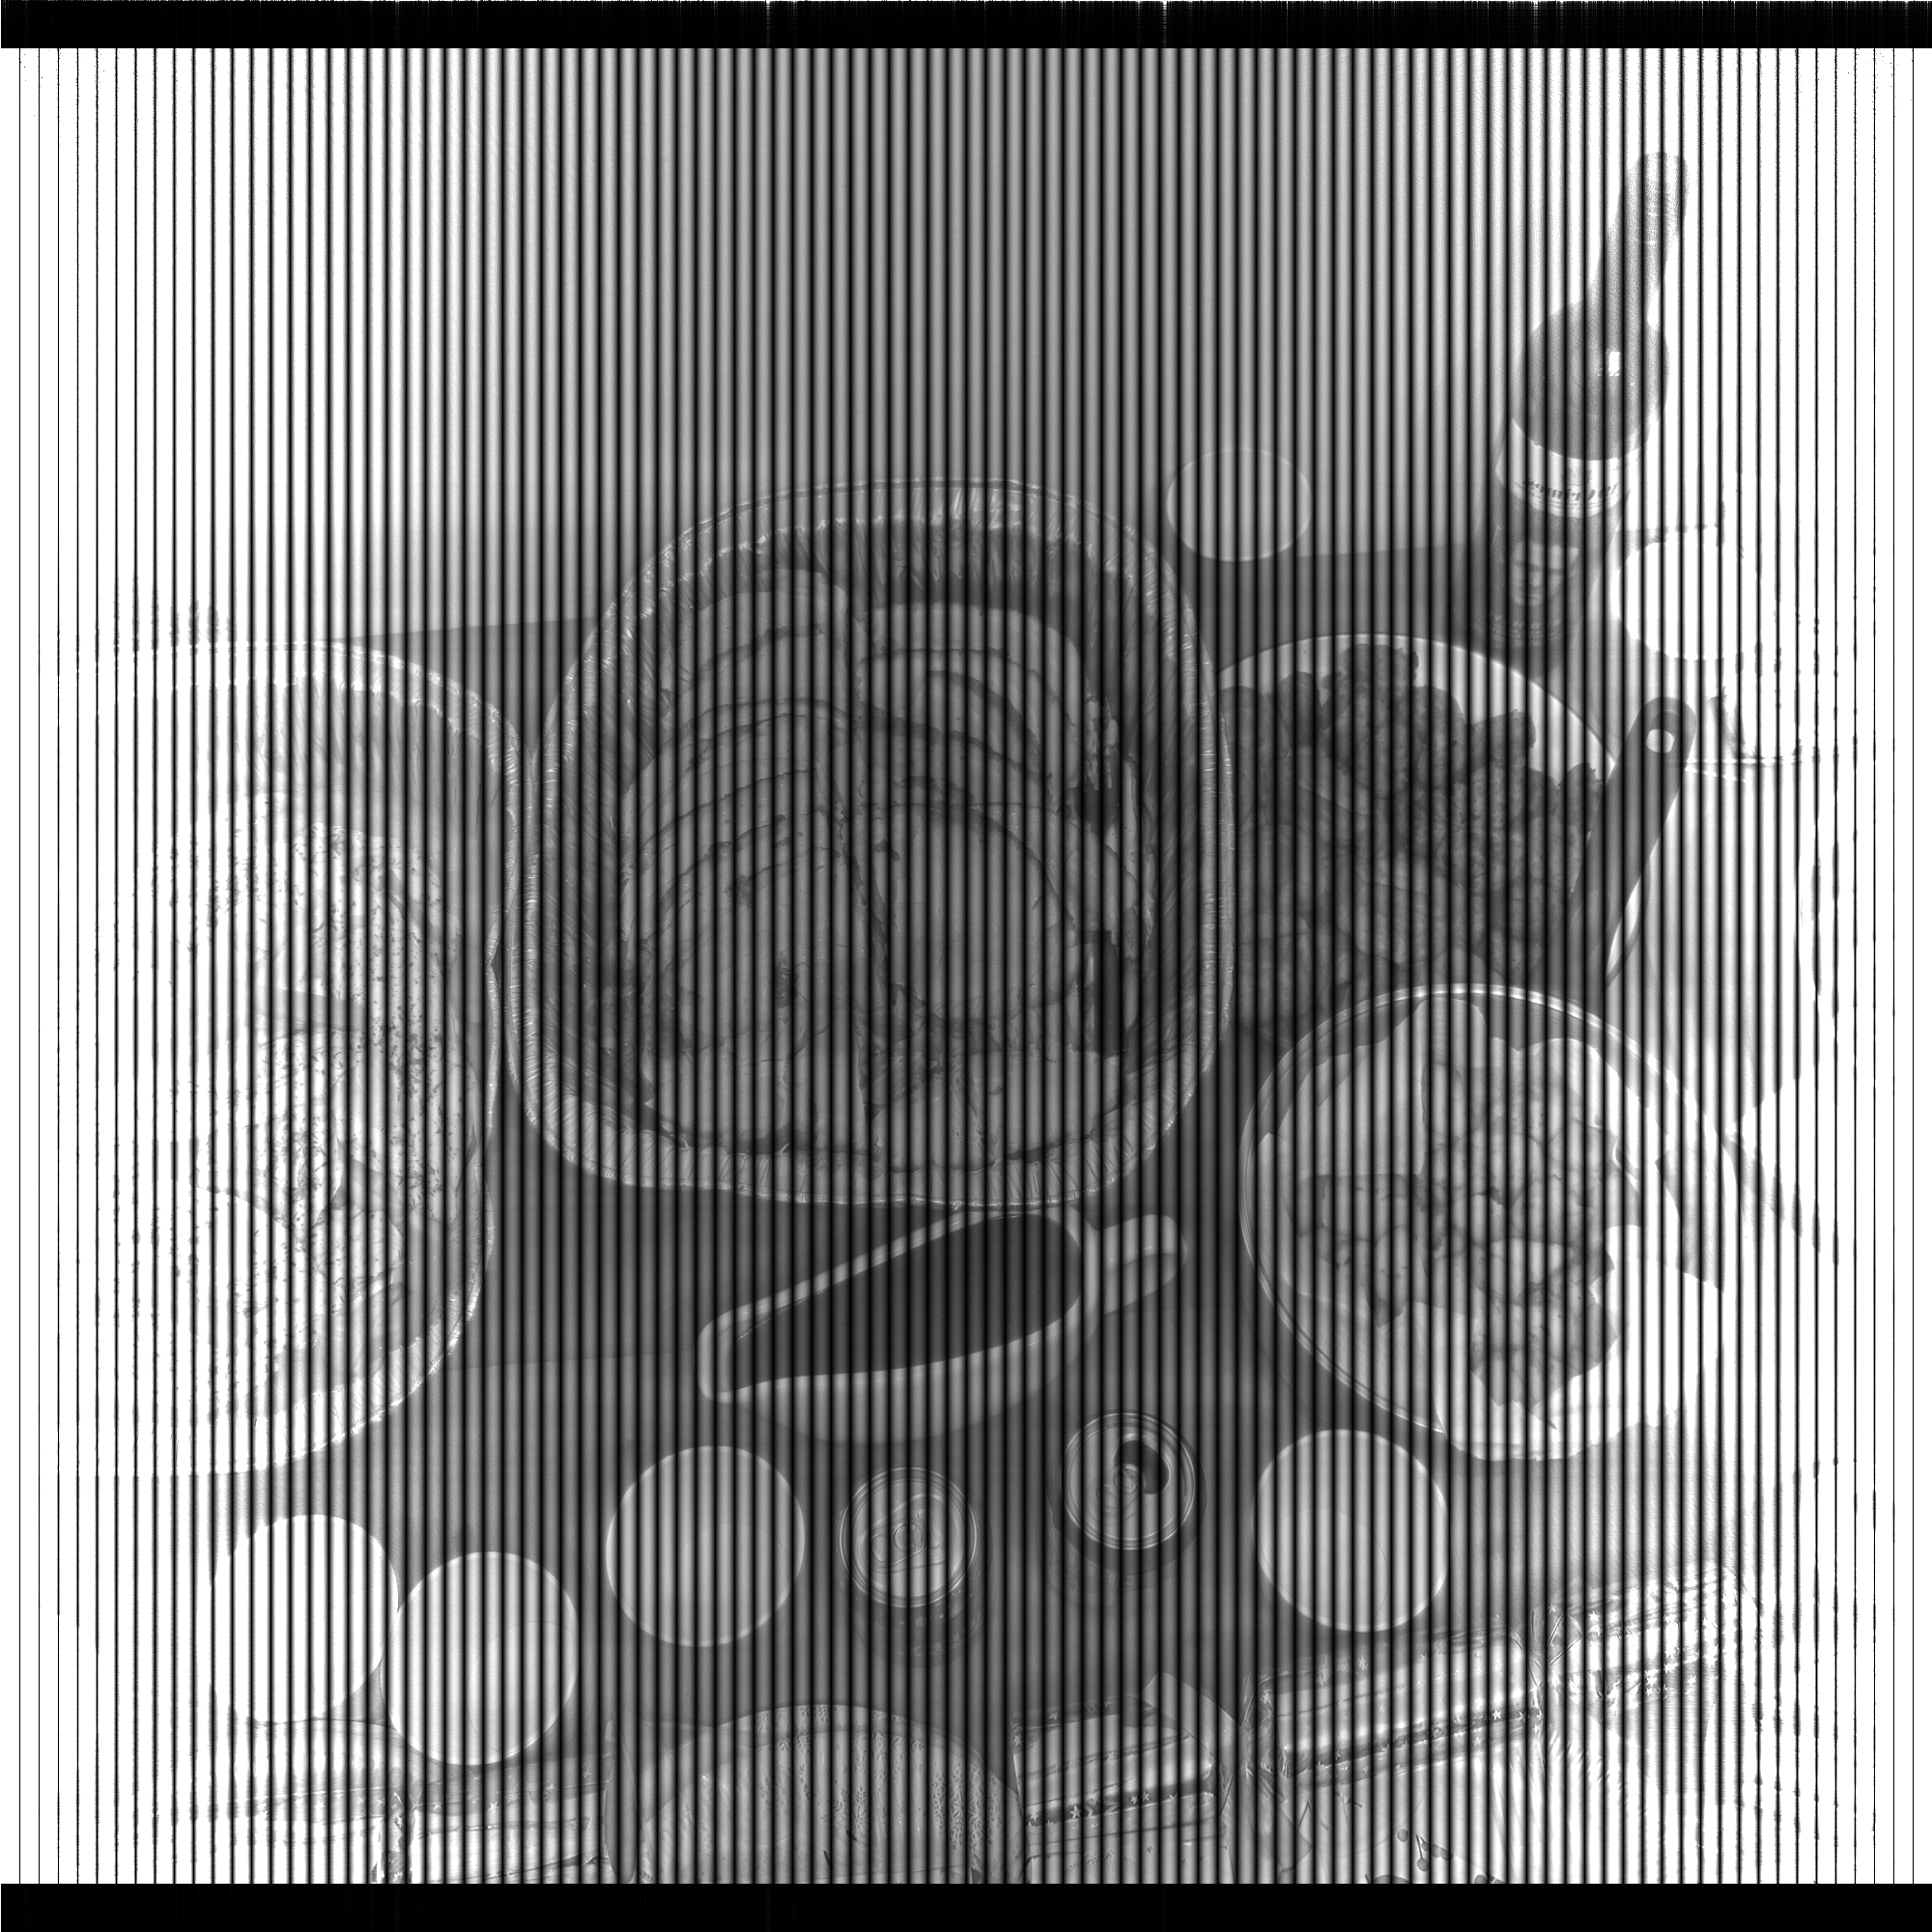
\includegraphics[width=0.5\textwidth]{double_inverse_fourier_image2.png}
\end{figure}

The convolution kernal I have created is a border image as shown in figure \ref{fig:box2}. I chose this because I noticed that the transformed image saw the pixels appearing to group on the edge, therefore I multiplied these to give them more focus. The result is visible in \ref{fig:fourierTransformFinal}

\pagebreak

\section{Final Code}

\lstinputlisting[language=C++]{../main.cpp}

\pagebreak

\printbibliography

\end{document}
